\documentclass[11pt]{article}


\usepackage{caption}

\usepackage{kotex}
\usepackage{sectsty}
\usepackage{graphicx}
\usepackage{amsmath}
\usepackage[margin=20mm]{geometry}
\usepackage{listings}
\usepackage{color}
\usepackage{lmodern} % Use a slightly nicer looking font
\usepackage{url} % Proper formatting for URLs
\usepackage{graphicx} % Handle inclusion of non-PDF graphics
\usepackage{subfig} % Allow sub-figures inside a figurexz
\usepackage{enumitem} % Allow lists to pick up numbering where the last list left off
\usepackage[margin=20mm]{geometry}
\usepackage{listings}
\usepackage{color}

\usepackage{setspace}
\setstretch{1.5} %간격 맞추는 패키지


% Color definitions for source code listings
\definecolor{mygreen}{rgb}{0,0.6,0}
\definecolor{mygray}{rgb}{0.5,0.5,0.5}
\definecolor{mymauve}{rgb}{0.58,0,0.82}

\lstset{ 
  backgroundcolor=\color{white},   % choose the background color; you must add \usepackage{color} or \usepackage{xcolor}
  basicstyle=\footnotesize,        % the size of the fonts that are used for the code
  breakatwhitespace=false,         % sets if automatic breaks should only happen at whitespace
  breaklines=true,                 % sets automatic line breaking
  captionpos=b,                    % sets the caption-position to bottom
  commentstyle=\color{mygreen},    % comment style
  deletekeywords={...},            % if you want to delete keywords from the given language
  escapeinside={\%*}{*)},          % if you want to add LaTeX within your code
  extendedchars=true,              % lets you use non-ASCII characters; for 8-bits encodings only, does not work with UTF-8
  frame=single,	                   % adds a frame around the code
  keepspaces=true,                 % keeps spaces in text, useful for keeping indentation of code (possibly needs columns=flexible)
  keywordstyle=\color{blue},       % keyword style
  otherkeywords={*,...},           % if you want to add more keywords to the set
  numbers=left,                    % where to put the line-numbers; possible values are (none, left, right)
  numbersep=5pt,                   % how far the line-numbers are from the code
  numberstyle=\tiny\color{mygray}, % the style that is used for the line-numbers
  rulecolor=\color{black},         % if not set, the frame-color may be changed on line-breaks within not-black text (e.g. comments (green here))
  showspaces=false,                % show spaces everywhere adding particular underscores; it overrides 'showstringspaces'
  showstringspaces=false,          % underline spaces within strings only
  showtabs=false,                  % show tabs within strings adding particular underscores
  stepnumber=2,                    % the step between two line-numbers. If it's 1, each line will be numbered
  stringstyle=\color{mymauve},     % string literal style
  tabsize=2,	                   % sets default tabsize to 2 spaces
  title=\lstname                   % show the filename of files included with \lstinputlisting; also try caption instead of title
}


% Margins
\topmargin=-0.45in
\evensidemargin=0in
\oddsidemargin=0in
\textwidth=6.5in
\textheight=9.0in
\headsep=0.25in


\title{Root Finding Homework 1}
\author{MinWook Kang}
\date{\today}

\begin{document}
\maketitle
\pagebreak

% Optional TOC
% \tableofcontents
% \pagebreak




%--Paper--
\section{scipy.optimize.root scalar Package를 이용한 예제 풀이}
\subsection{Cube Root} 

우리는 먼저 scipy.optimize.root scalar package 를 필요가 있다. 이는 scipy의 한 모듈로, 뉴턴의 방식을 예로 들자면,
\vspace{5mm}
\begin{lstlisting}[language=Python]
from scipy import optimize
sol = optimize.root_scalar(f, x0 = 1, fprime = df, method = 'newton')
\end{lstlisting}

\noindent
와 같은 방법으로 불러올 수 있다. optimize 에는 다양한 방법으로 근을 근사할 수 있는 모듈을 제공하는데, 모듈에 따라optimize.root scalar 에 필요한 인수의 값이 달라지게 된다.  우선 먼저 Cube Root 를 Newton's Method 로 풀어보겠다. 문제는 다음과 같다.
\begin{equation}
 x^3  -  2 =  0
\end{equation}

\noindent
이 문제를 풀기 위해서, 우선 optimize 모듈을 불러와서 모듈을 실시하기 위해 필요한 parameter 인 함수 $f$ 와 초기값 $x_0$ = 1, 그리고 도함수인 $f'$ 을 구해야 한다. 이때 함수는 제시된 함수를 대입하면 되고, Newton's Method 에서 가장 중요한 초기값을 선택해야 하는데, 이는 $x^3 - 2 = 0$ 의 식에서, 해와 비슷할 것 같은 값중 정수인 1을 대입하여 구하였다.  이를 Python 으로 구현하면,
\vspace{5mm}
\lstinputlisting[language=Python, firstline=7, lastline=31]{CubeRoot_Homework1.py}
\vspace{5mm}

\noindent
$(1.2599210498948732)$ 가 출력 된다. 이때, optimize 에서는 root, iterations-반복횟수를 나타낸다. 

\subsection{Golden Ratio} 
이와 같은 방법으로 다른 문제에도 접근해보자. Golden Ratio를 구하는 문제이다. 먼저 Golden Radio 는 우리가 아래의 $\phi$로 근사하는데
$$
\phi = \frac{1 + \sqrt 5}{2} \approx 1.6180339887498948482
$$
\noindent
이는 $f(x) \equiv x^2 - x - 1 = 0$의 해로 근사할 수 있고 이를 푸는 문제를 Python으로 구현하면,

\vspace{5mm}
\lstinputlisting[language=Python, firstline=7, lastline=31]{Golden_Ratio_Homework1.py}
\vspace{5mm}

\subsection{Supergolden Ratio} 
\noindent
앞에서는 bisect의 방법으로 문제를 풀었다. 이때, bisect에서 중요한 parameter인 bracket은 범위를 뜻하는 것이고, 이는 $[1, 2]$로 대략적이게 추산하였다. 위에서 말한 초기값이나 범위를 이렇게 잡은 이유에 대해서는 후에 다른 문제를 풀면서 그래프를 이용하여 더 자세히 다룰 것이다. 비슷한 문제로 Supergolden Ratio의 값을 추산하면, 

\vspace{5mm}
\lstinputlisting[language=Python, firstline=7, lastline=31]{Supergolden_Ratio_Homework1.py}
\vspace{5mm}

$$
\psi = \frac{1 + \sqrt[3]{\frac{29 + 3\sqrt{93}}{2}} + \sqrt[3]{\frac{29 - 3\sqrt{93}}{2}}}{3}
\approx 1.4655712318763108
$$

\subsection{Zeros of Bessel Functions} 
\noindent
이제는 조금 다르게, 예제들에서 있던 Bessel 함수에서 optimize 를 통해 구한 근을 직접 그래프로 표시하여 optimize 에서 추산한 솔루션이 실제 값과 비슷한지를 시각적으로 표현해 볼 것이다. 먼저 이미 선행으로 알려진 Bessel 함수의 코드는 다음과 같다.

\begin{lstlisting}[language=Python]
intervals = (0, 5, 7, 10, 13, 16, 20, 23, 25, 28)
x_zeros = [bisection_while(lambda x: special.jn(0, x), ab,
                    lambda i, xy, dx: abs(xy[1]) >= 1e-10)
    for ab in zip(intervals[:-1], intervals[1:])]
\end{lstlisting}


\clearpage
\begin{figure}[!ht]
  \centering
  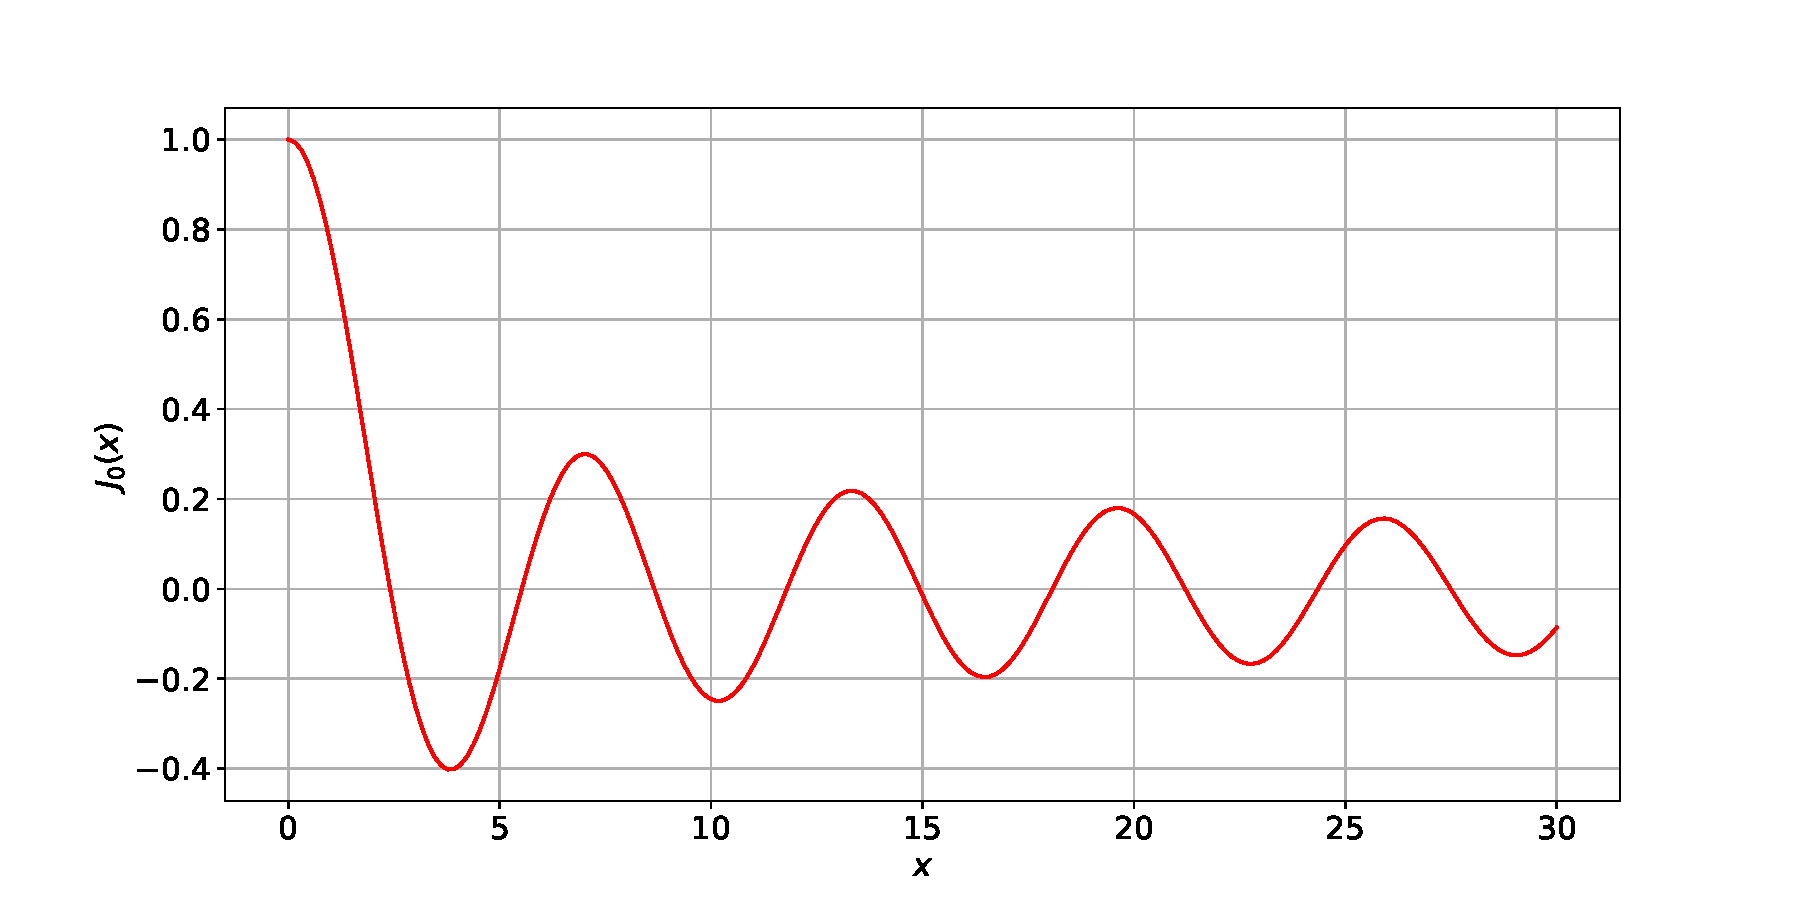
\includegraphics[width=0.5\textwidth]{Bessel_Functions.pdf}
  \caption{Bessel Function}
\end{figure}

\noindent
 위의 그래프에서 점을 찍는 코드를 optimize 를 통해 구현할 것이다. 미리 알려진 코드에서는 intervals 와 x-zeros에 대한 코드를 튜플과 리스트 내포를 이용하여 나타내었지만, 이를 for 문과 append 함수를 통해서 그래프를 만들어 보았다.
 
\vspace{5mm}
\lstinputlisting[language=Python, firstline=32, lastline=51]{Zeros_of_Bessel_Fuctions_Homework1.py}
\vspace{5mm}

\noindent
이를 그래프로 나타내면, 아래와 같다.

\begin{figure}[!ht]
  \centering
  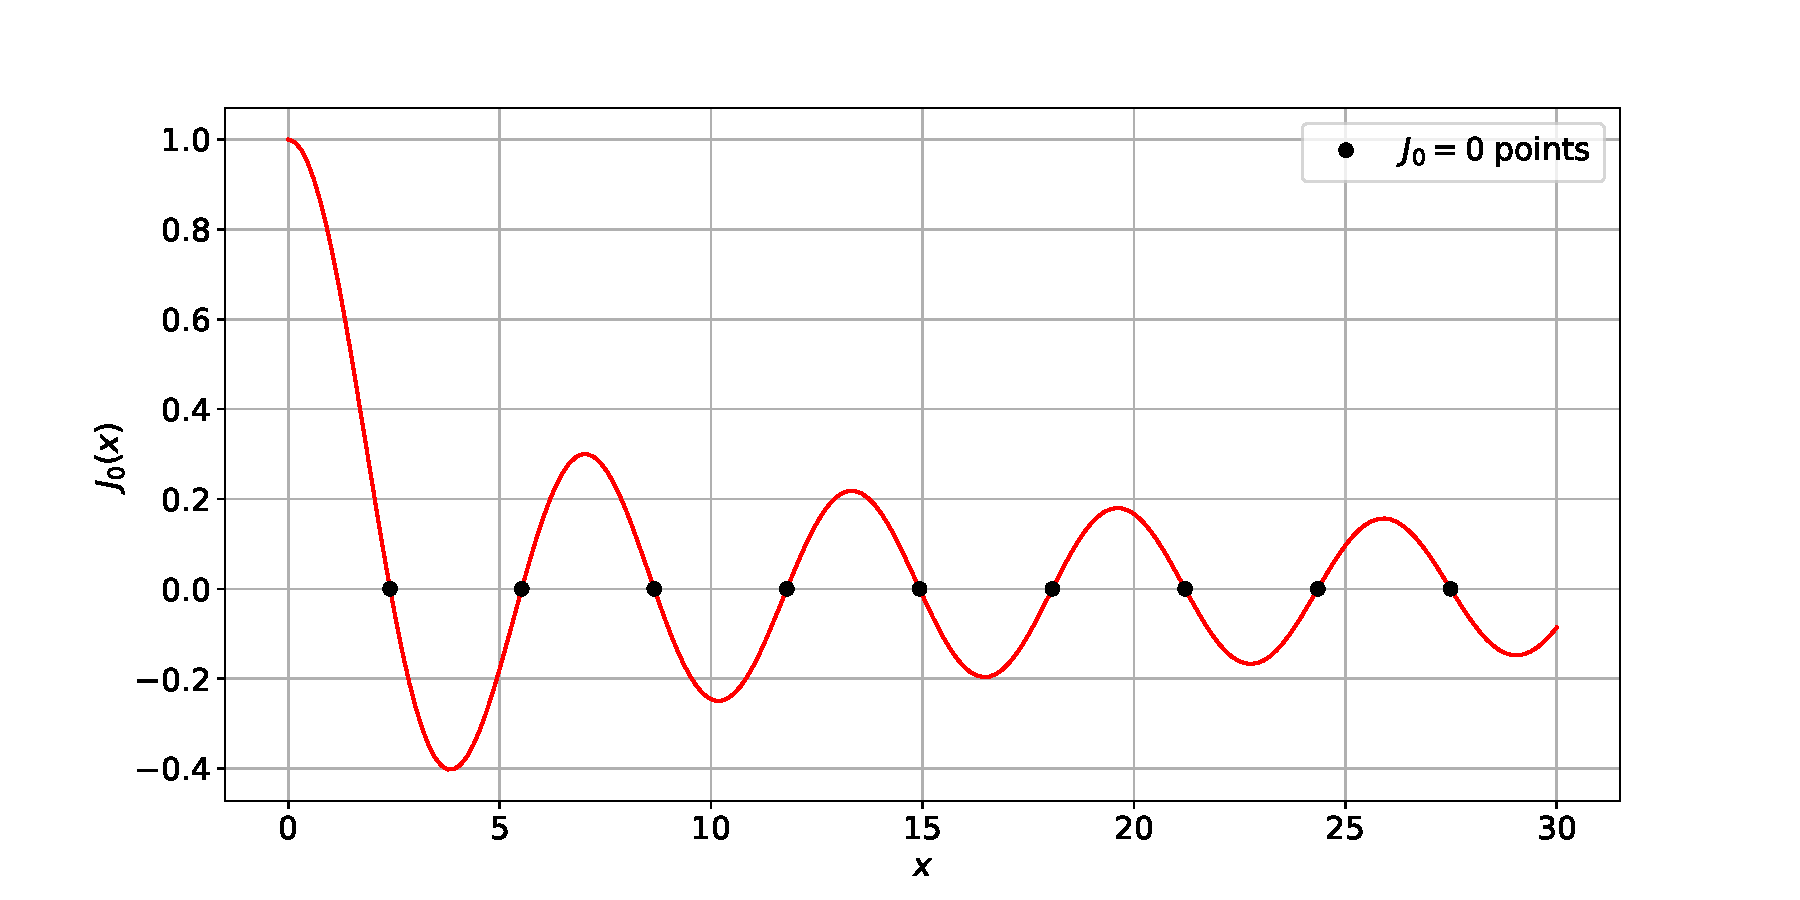
\includegraphics[width=0.5\textwidth]{Zeros_of_Bessel_Fuctions_Homework1.pdf}
  \caption{Bessel Function's Zero points}
\end{figure}
\clearpage














\section{Root Finding by Coding}
\subsection{Bisection Method} 
\noindent
이번에는, 아래의 함수를 전산수치 및 실습의 강의록에서 def 함수를 통해 만들어진 코드들을 응용하여 문제를 풀어보겠다. 주어진 조건에 따라서 4가지 방법(Bisection, Muller, Newton, Secant) 를 풀어볼 것이다. 먼저 세 가지의 함수를 정의하면 다음과 같다. 
\begin{equation}
f_1(x) = sin(x) - x - 1
\end{equation}
\begin{equation}
f_2(x) = x(1 - cos(x))
\end{equation}
\begin{equation}
f_3(x) = e^{x} - x^2 + 3x - 2 
\end{equation}

\noindent
그리고 Bisection Method 의 코드를 잠시 보여주면 다음과 같은데, 이 함수를 그대로 이용하되, 우리는 return에서 iteration값을 알아야 하기에, 두가지 값을 볼 수 있도록 return값을 $i$ 와 $x_{mid}$의 튜플로 나타내었다.

\begin{lstlisting}[language=Python]
def bisection_while(f, xinit, predicate):
    a_n, b_n = xinit
    f_1st = f(a_n)

    if f(a_n) * f(b_n) >= 0:
        print("Bisection method fails.")
        return None

    i = 1
    x_mid = 0.5 * (a_n + b_n)
    f_mid = f(x_mid)
    while predicate(i, (x_mid, f_mid), 0.5 * abs(a_n - b_n)):
        if f_1st * f_mid > 0:
            a_n = x_mid
            f_1st = f_mid
        else:
            b_n = x_mid

        i = i + 1
        x_mid = 0.5 * (a_n + b_n)
        f_mid = f(x_mid)
        

    return i, x_mid
\end{lstlisting}

\noindent
알려진 코드에서 $f_1$, $f_2$, $f_3$ 각각에 해당하는 $x$에 대한 함수로 나타내고, 이때 주어진 조건에 맞게 parameter을 정할 것이다. 우선 첫번째, Bisection Method에서는 interval 을 $(-2, 1)$ 로 두고, 절대 오차로부터 $10^{-6}$ 정도의 차이가 날 수 있도록 조정하기 위하여, lambda 함수의 절댓값 오차를 수정한다. 즉, 원하는 값을 수정하여 값을 추산하고 우리가 원하는 iteration 값과 approx solution 값을 추산하면 다음과 같다.

\begin{lstlisting}[language=Python]
f_1_approx_bisection = bisection_while(lambda x: np.sin(x) - x - 1, (-2,1), 
									lambda i, xy, dx: abs(dx) > 1e-6)
print(f"iteration: {f_1_approx_bisection[0]}, approx solution: {f_1_approx_bisection[1]}") 
Output : iteration: 22, approx solution: -1.934563398361206
\end{lstlisting}


\begin{lstlisting}[language=Python]
#f_2(x) approx
f_2_approx_bisection = bisection_while(lambda x: x * (1 - np.cos(x)), (-2,1),
                                   lambda i, xy, dx: abs(dx) > 1e-6)
print(f"iteration: {f_2_approx_bisection[0]}, approx solution: {f_2_approx_bisection[1]}")
Output : iteration: 22, approx solution: 2.384185791015625e-07
\end{lstlisting}

\begin{lstlisting}[language=Python]
#f_3(x) approx
f_3_approx_bisection = bisection_while(lambda x: np.exp(x) - x**2 + 3 * x - 2, (-2,1),
                                   lambda i, xy, dx: abs(dx) > 1e-6)
print(f"iteration: {f_3_approx_bisection[0]}, approx solution: {f_3_approx_bisection[1]}")
Output : iteration: 22, approx solution: 0.25753092765808105
\end{lstlisting}












\subsection{Secant Method} 
\noindent 
Secant Method 도 같은 방식으로 위와 같은 방식으로 return에 대한 값만 수정하여 iteration을 구할 수 있도록 수정하였다.  

\begin{lstlisting}[language=Python]
f_1_approx_secant = secant_while(lambda x: np.sin(x) - x - 1, (-2,1), 
                   		lambda i, xy, dx: abs(dx) > 1e-6)
print(f"iteration: {f_1_approx_secant[0]}, approx solution: {f_1_approx_secant[1]}")
Output : iteration: 7, approx solution: -1.9345632107519628
\end{lstlisting}

\begin{lstlisting}[language=Python]
f_2_approx_secant = secant_while(lambda x: x * (1 - np.cos(x)), (-2,1), 
                                   lambda i, xy, dx: abs(dx) > 1e-6)
print(f"iteration: {f_2_approx_secant[0]}, approx solution: {f_2_approx_secant[1]}")
Output : iteration: 45, approx solution: 2.5551058010235595e-06
\end{lstlisting}

\begin{lstlisting}[language=Python]
f_3_approx_secant = secant_while(lambda x: np.exp(x) - x**2 + 3 * x - 2, (-2,1), 
                                   lambda i, xy, dx: abs(dx) > 1e-6)
print(f"iteration: {f_3_approx_secant[0]}, approx solution: {f_3_approx_secant[1]}")
Output : iteration: 5, approx solution: 0.2575302854397244
\end{lstlisting}

\noindent 
이때, 범위 대신, 문제에서 주어진 $x_0$ 과 $x_1$ 값을 이용하여 값을 추산할 수도 있는데, 이러면 secant while 함수가 아닌 secant by 함수를 사용하여야 한다. 이는 당연하게도, parameter에서 xinit(범위) 가 아닌, a, b 을 따로 받아서 함수에 적용하기 때문에, $ a = x_0 $, $b = x_1 $으로 이해할 수 있다. 이를 Python으로 나타내면, 

\begin{lstlisting}[language=Python]
f_1_approx_secant_by = secant_by(lambda x: np.sin(x) - x - 1, 1, 0.9,
                                   9)
print(f"iteration: {f_1_approx_secant_by[0]}, approx solution: {f_1_approx_secant_by[1]}")
Output :iteration: 9, approx solution: -1.9345632107520243
\end{lstlisting}

\begin{lstlisting}[language=Python]
f_2_approx_secant_by = secant_by(lambda x: x * (1 - np.cos(x)), 1, 0.9,
                                   45)
print(f"iteration: {f_2_approx_secant_by[0]}, approx solution: {f_2_approx_secant_by[1]}")
Output :iteration: 45, approx solution: 2.6043552455913054e-06
\end{lstlisting}

\begin{lstlisting}[language=Python]
f_2_approx_secant_by = secant_by(lambda x: (np.exp(x) - x**2 + 3 * x - 2), 1, 0.9,
                                   6)
print(f"iteration: {f_2_approx_secant_by[0]}, approx solution: {f_2_approx_secant_by[1]}")
Output :iteration: 6, approx solution: 0.2575302854398608
\end{lstlisting}












\subsection{Muller's Method} 


Muller's Method 를 사용할 때에는 조심스러운 부분이 있다. 바로 초기 값에 따라 값이 크게 달라질 수 있다는 것이다. 또한 초기값이 총 세개여야 하므로, 이를 구하는 것이 중요한 방법이라고 볼 수 있다. 위의 방법대로 범위를 정하고, 문제에서 주어진 초기값 $x_0 = 1$, $x_1 = 0.9$, $x_2 = 0.95$ 를 parameter에 각각 대입하여 문제를 푼다.

\begin{lstlisting}[language=Python]
f_1_approx_muller = muller_while(lambda x: np.sin(x) - x - 1, (1, 0.9, 0.95), 
                           lambda i, xy, dx: abs(xy[1]) > 1e-6 or i > 500)
print(f"iteration: {f_1_approx_muller[0]}, approx solution: {f_1_approx_muller[1]}")
Output : iteration: 5, approx solution: (0.816463531131045-1.5635846377499045j)
\end{lstlisting}

\begin{lstlisting}[language=Python]
f_2_approx_muller = muller_while(lambda x: x * (1 - np.cos(x)), (1, 0.9, 0.95), 
                           lambda i, xy, dx: abs(xy[1]) > 1e-6 or i > 500)
print(f"iteration: {f_2_approx_muller[0]}, approx solution: {f_2_approx_muller[1]}")
Output : iteration: 14, approx solution: (-0.006364773235289123-0.007825774561814524j)
\end{lstlisting}

\begin{lstlisting}[language=Python]
f_3_approx_muller = muller_while(lambda x:  np.exp(x) - x**2 + 3 * x - 2, (1, 0.9, 0.95), 
                           lambda i, xy, dx: abs(xy[1]) > 1e-6 or i > 500)
print(f"iteration: {f_3_approx_muller[0]}, approx solution: {f_3_approx_muller[1]}")
Output : iteration: 4, approx solution: (0.257530285446518+0j)
\end{lstlisting}













\subsection{Newton's Method} 


Newton's Method 를 고려할 때에는 초기값 뿐만 아니라, 도함수 $f'(x)$ 도 고려해야 한다. 따라서 이를 원래의 $f(x)$ 함수를 미분하여 계산해야하므로 앞선 방법과 달리 조금 복잡할 수 있지만, 도함수를 구하기 쉬운 경우에는 가장 빠르게 해를 접근할 수 있는 방식 중에 하나이다. 하지만 초기 값에 따라 근처의 해를 도출하는 탓에 진동하는 그래프의 경우, 초기값에 따라서 근처의 값이 아닌 완전 다른 값을 추산해 낼 수 있다. 이 이유는 접선의 방정식이 만드는 $g(x) = 0$을 만드는 $x$ 값에 따라 접선의 기울기가 작을 수록 더 멀리 떨어진 $x$ 값을 추산하기 때문에 발생하는 원인이다. 

또한 두번째 문제점은 후에 논의할 진동하는 함수의 경우 (예를 들어 위에서 본 Bessel Functions 처럼) 접선의 기울기가 무한대에 수렴할 경우, iteration이 끊임없이 증가하게 되면서 함수가 무한히 반복되는 경우가 생길 수 있다. 그렇기에 우리는 앞선 방식과 달리, 함수를 불러왔을 때, 제한 조건을 걸어 $abs(dx)$, 즉 절대 오차의 한계를 줄 뿐만아니라, iteration의 한계를 걸어서 에러가 발생하는 것을 막아야 한다. 하지만 이럼에도 뒤에 나올 $f_2(x)$ 에서는 오류가 발생한다. 먼저 $f_1(x)$ 과  $f_2(x)$ 함수의 해를 근사적으로 구해보자.
\vspace{5mm}

\begin{lstlisting}[language=Python]
iterations = -1
def predicate(i, xy, dx):
    global iterations
    iterations = i
    print("\ti = {}, xy = {}, dx = {}".format(i, xy, dx))
    return abs(dx) > 1e-6 and i < 500 

f_1_approx_newton = newton_while(lambda x : (np.sin(x) - x - 1,np.cos(x)-1), 
                        1, predicate)

if iterations >= 500:
    print(f"\n!! Exeeded maximum iterations (={500}) befor convergence !!")
    
print(f"iteration: {f_1_approx_newton[0]}, approx solution: {f_1_approx_newton[1]}")

Output : i = 1, xy = (1, -1.1585290151921035), dx = -2.520197577627591
	i = 2, xy = (-1.5201975776275911, -0.4785225787569186), dx = -0.5040141854424416
	i = 3, xy = (-2.0242117630700327, 0.12525550683758802), dx = 0.08710164199542941
	i = 4, xy = (-1.9371101210746033, 0.003456123890821061), dx = 0.002544679996650069
	i = 5, xy = (-1.9345654410779534, 3.0238718413677645e-06), dx = 2.230324214770129e-06
	i = 6, xy = (-1.9345632107537385, 2.3241408797503027e-12), dx = 1.7142246509540634e-12
iteration: 6, approx solution: -1.9345632107520243
\end{lstlisting}

\begin{lstlisting}[language=Python]
iterations = -1
def predicate(i, xy, dx):
    global iterations
    iterations = i
    print("\ti = {}, xy = {}, dx = {}".format(i, xy, dx))
    return abs(dx) > 1e-6 and i < 500 #iteration can not 500

f_3_approx_newton = newton_while(lambda x :   ((np.exp(x) - x**2 + 3 * x - 2), np.exp(x) - 2 * x + 3), 
                        1, predicate)

if iterations >= 500:
    print(f"\n!! Exeeded maximum iterations (={500}) befor convergence !!")
    
print(f"iteration: {f_3_approx_newton[0]}, approx solution: {f_3_approx_newton[1]}")
	i = 1, xy = (1, 2.7182818284590446), dx = -0.7310585786300048
	i = 2, xy = (0.2689414213699952, 0.04307326004788026), dx = -0.011423160112898526
	i = 3, xy = (0.2575182612570967, -4.543547480073684e-05), dx = 1.2024169252108878e-05
	i = 4, xy = (0.2575302854263488, -5.1057158501066624e-11), dx = 1.3511937484935972e-11
iteration: 4, approx solution: 0.25753028543986073
\end{lstlisting}

\noindent  
다른 방법으로 구한 해를 통해서 두 가지의 해 모두 정상적으로 들어 맞는 것을 볼 수 있다. 하지만 $f_2(x)$ 는 다음과 같은 오류가 발생한다. 

\begin{lstlisting}[language=Python]
iterations = -1
def predicate(i, xy, dx):
    global iterations
    iterations = i
    print("\ti = {}, xy = {}, dx = {}".format(i, xy, dx))
    return abs(dx) > 1e-6 and i < 500 

solution = newton_while(lambda x :  (x * (1 - np.cos(x)), 1 - (np.cos(x) + x * np.sin(x))), 
                    1, predicate)

if iterations >= 500:
    print(f"\n!! Exeeded maximum iterations (={500}) befor convergence !!")
    
print(solution) 
Output : i = 500, xy = (128.98670583780643, 255.85684522781344), dx = -10.131114683075353

!! Exeeded maximum iterations (=500) befor convergence !!
(500, 118.85559115473107)
\end{lstlisting}

\noindent  
이와 관련해서는 다음의 Three Question Chapter 의 2번 문제에서 다뤄보도록 할 것이다. 사실 이것은 오류가 아니다. 이 코드는 $iteration \geq 500$ 이 될 경우 위에 식에 있는 아래의 코드에 의해 코드를 중단하고 그 때의 해를 보여주면서 무한 루프를 피하기 위해 만들어졌다.
\begin{lstlisting}[language=Python]
if iterations >= 500:
    print(f"\n!! Exeeded maximum iterations (={500}) befor convergence !!")
\end{lstlisting}

























이제는 아래의 질문에 답을 적어보겠다.
\vspace{2mm}
\begin{enumerate}
\item Why did the bisection method require approximately the same number of iterations to converge to the approximate root for all three test problems?
\item Newton’s method should have experienced difficulty approximating the root of one of the test functions (when using 
$x_0 = 1$). Identify which function presented a problem and explain why the difficulty occurred.
\item  Above you used the bisection method to find the root of the function $f_1(x) = \sin(x) -  x - 1$. Consider the function $g_1(x) =( \sin(x) - x - 1 )^2$. Clearly $f_1(x)$ and $g_1(x)$ have the same root in $x \in [-2, 1]$. Could the bisection method be used to numerically approximate the root of $g_1(x)$? Why or why not?
\end{enumerate}
\vspace{2mm}

\subsection{First Question} 
\noindent  
1번 문제는 Bisection 방식을 통해서 해를 근사적으로 구할 경우, iteration 값이 동일 한 것에 대해서 물어보는 문제이다. Bisection 방식은 어떤 값을 찾는 프로그래밍에서 사용하는 알고리즘에서 많이 쓰이는 이분 탐색과 원리가 같다. 즉, 이진 탐색에서는 한 번 비교할 때마다 탐색의 범위가 절반으로 줄어드는 것 처럼, Bisection Method 또한 그러하다. 
\begin{figure}[!ht]
  \centering
  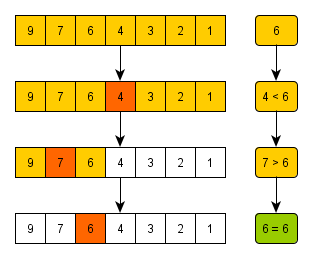
\includegraphics[width=0.5\textwidth]{Bisection_method.png}
  \caption{이진 탐색 알고리즘의 예}
\end{figure}


따라서 해를 구할때, 절대 오차 크기 까지의 범위를 찾으려면 그 단위 만큼 잘라내는 단계가 필요하다. 우리가 원하는 절대 오차의 크기는 $10^{-6}$ 이다. 이정도의 간격 만큼 잘라내는 단계는 $2^{-22}$ 번 이상이 될 경우 절대 오차의 크기보다 더 작아지게 되면서 함수가 끝나게 된다. 이를 직접 증명하는 방식은, 사실 1e-6 대신 1e-7을 대입하면 solution이 달리짐을 볼 수 있는데, 이는 달라진 절대 오차의 크기만큼 해를 더 잘게 잘라내기 때문에 잘라낸 만큼 절대 오차에 가까울 수 있도록 이진 탐색을 계속해서 진행하면서 iteration이 25만큼 늘어난다. 다음 코드를 보자. 
\begin{lstlisting}[language=Python]
#f_2(x) approx
f_2_approx_bisection = bisection_while(lambda x: x * (1 - np.cos(x)), (-2,1),
                                   lambda i, xy, dx: abs(dx) > 1e-7)
print(f"iteration: {f_2_approx_bisection[0]}, approx solution: {f_2_approx_bisection[1]}")
Output : iteration: 25, approx solution: -2.9802322387695312e-08
\end{lstlisting}
\noindent  
앞에서 본 코드와 달리 solution은 더 정확해 졌지만 (이는 절댓값의 크기를 통해 알 수 있다.) , iteration은 25번으로 많아졌다. 또한 아래의 그림처럼 절대 오차는 count가 증가할 수록 작아지면서 $f(x_n)$ 의 값 또한 줄어 드는 것을 만족한다. 
\begin{figure}[!ht]
  \centering
  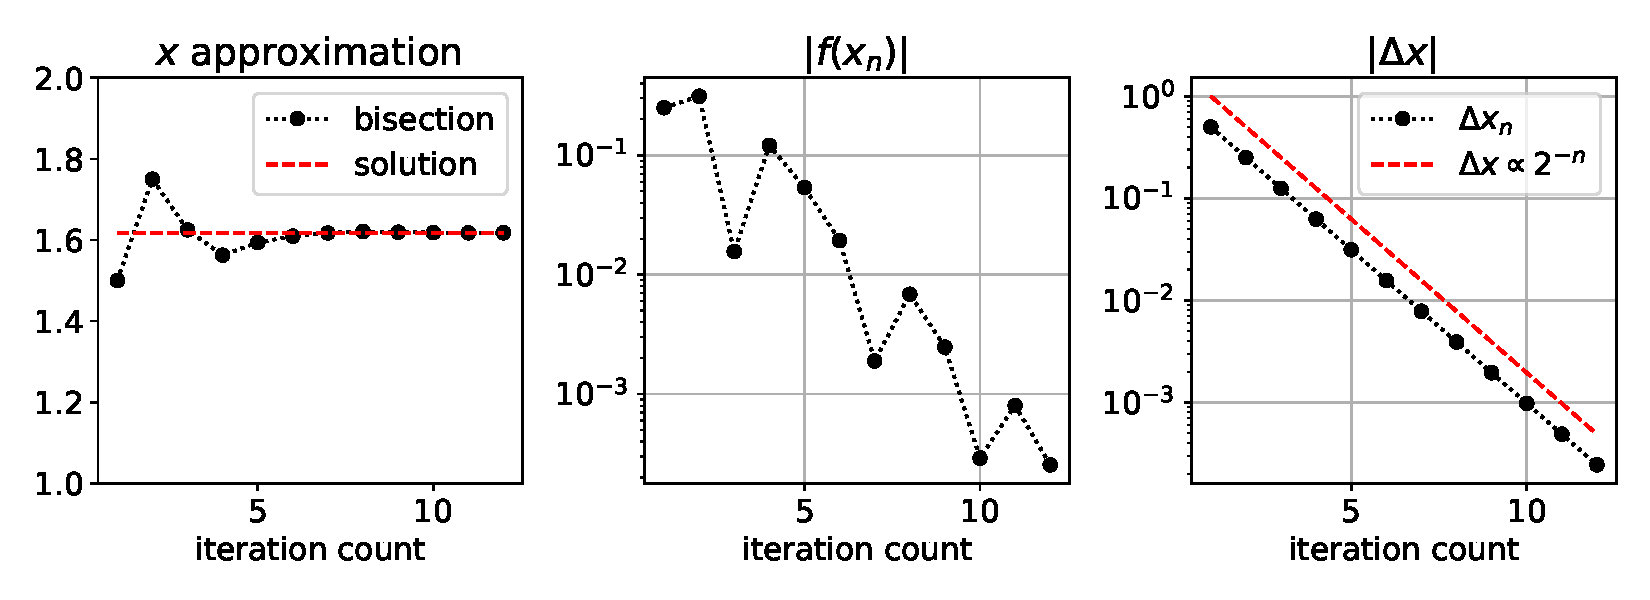
\includegraphics[width=1\textwidth]{bisection_sol_Method_approximation.pdf}
  \caption{$x$ approximation with real solution}
\end{figure}

\noindent  
부호가 바뀌는 것은 이 함수의 경우 진동하는 함수이기 때문에 이 함수를 그리게 되면 그 이유에 대해서 추측할 수 있다. 

\begin{figure}[!ht]
  \centering
  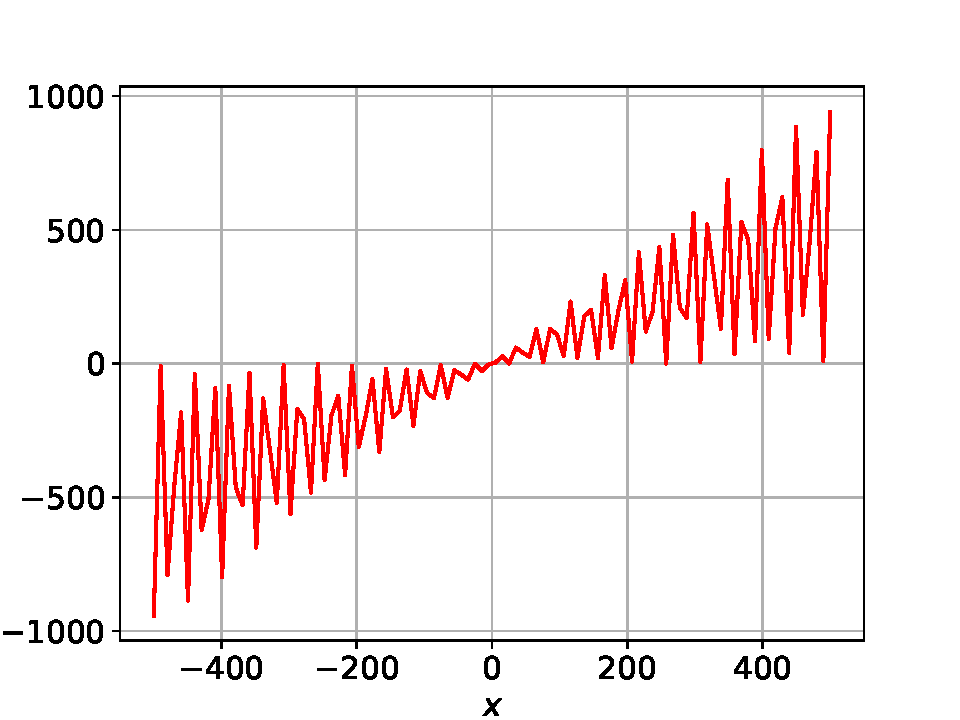
\includegraphics[width=0.7\textwidth]{f_2(x).pdf}
  \caption{$f_2(x)$ Graph}
\end{figure}

그래프가 진동하는 형상을 볼 수 있다. 이러한 상황에서 Bisection Method 의 조건인 $f(a)f(b) < 0 $ 을 만족하면 제한된 조건하에, 계속하여 해를 구할 수 있기 때문에 어느 정도의 구체적인 해를 얻기전의 iteration 번째 전에는 부호가 바뀔 수 있다.













\subsection{Second Question} 
아까 위에서 진동하는 함수의 경우 접선의 기울기가 무한대에 수렴할 경우, iteration이 끊임없이 증가하게 되면서 함수가 무한 반복되는 경우를 볼 수 있었다. 그리고 이를, iteration의 한계를 걸어줌으로써 문제를 차단했지만, 그럼에도 해가 갑자기 늘어나는 경우가 발생했다. 사실 이는, Newton's Method의 단점 중 하나이다. 진동하는 해의 경우 해가 잘못 도출될 수 있는 것인데, 이를 확인하기 위하여 아래의 그래프를 보면,
\begin{figure}[!ht]
  \centering
  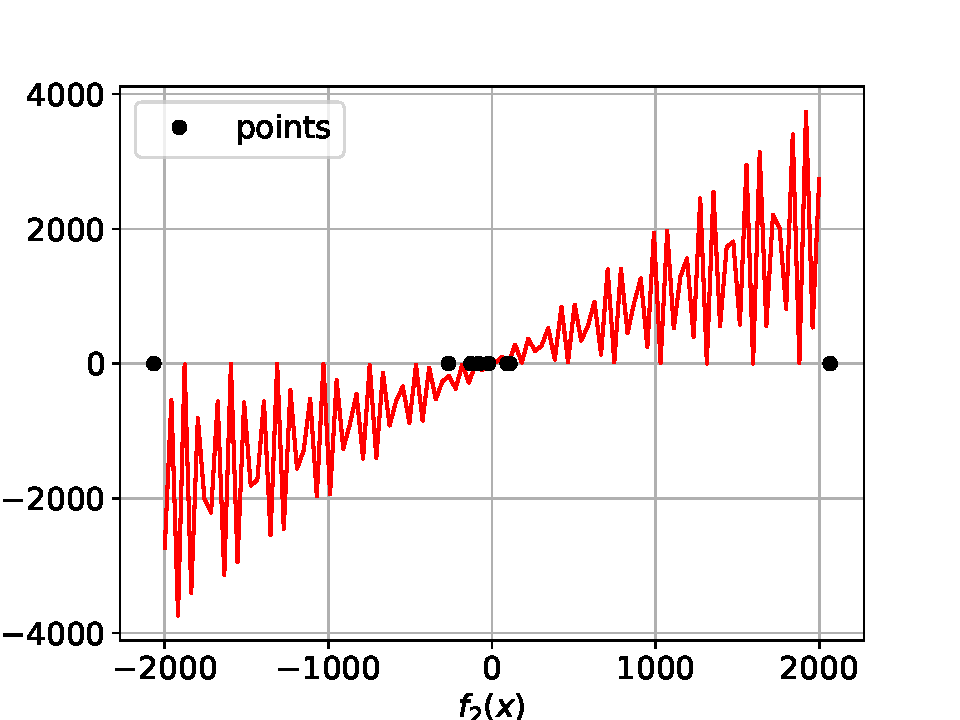
\includegraphics[width=0.7\textwidth]{Newtown_Method_strange.pdf}
  \caption{Newton Method Graph and  $X_{zeors}$}
\end{figure}


\begin{lstlisting}[language=Python]
intervals = np.linspace(-20, 20, 10)

x_zeros = []
def f(x):
    return x * (1 - np.cos(x))

def fprime(x):
    return 1 - (np.cos(x) + x * np.sin(x))


for ab in zip(intervals[:-1], intervals[1:]):
    sol = optimize.root_scalar(f, fprime = fprime , bracket=ab, method='newton', x0 =ab[1])
    x_zeros.append(sol.root)

x = np.linspace(-2000, 2000, 100)
y = x * (1 - np.cos(x))

plt.figure()
plt.plot(x, y, '-r')
plt.plot(x_zeros, np.zeros_like(x_zeros), 'ok',
         label="points")
plt.xlabel("$f_2(x)$")
plt.ylabel("$function$")
plt.grid()
plt.legend()
plt.savefig("Newtown_Method_strange.pdf")
\end{lstlisting}

\noindent  
Figure 6의 검은색 point는 Newton's Method를 optimize로 계산한 해를 구한 것이다. 여기서도 볼 수 있듯이,  해가 갑자기 뜬 경우를 볼 수 있고, 이것이 Newton's Method의 단점 중 하나라고 볼 수 있다. 즉 이는 초기값에 따라서 값이 달라질 수 있다는 것이고, $f'(x)$ 이 0 에 한없이 가까워 질수록 무한히 반복할 수 있다.
\clearpage










\subsection{Thrid Question} 
이는 위에서 잠시 소개한 Bisection Method의 특징 때문이다. 우선 $g_1(x)$ 그래프를 그리게 되면 Figure 7과 같다. 
\begin{figure}[!ht]
  \centering
  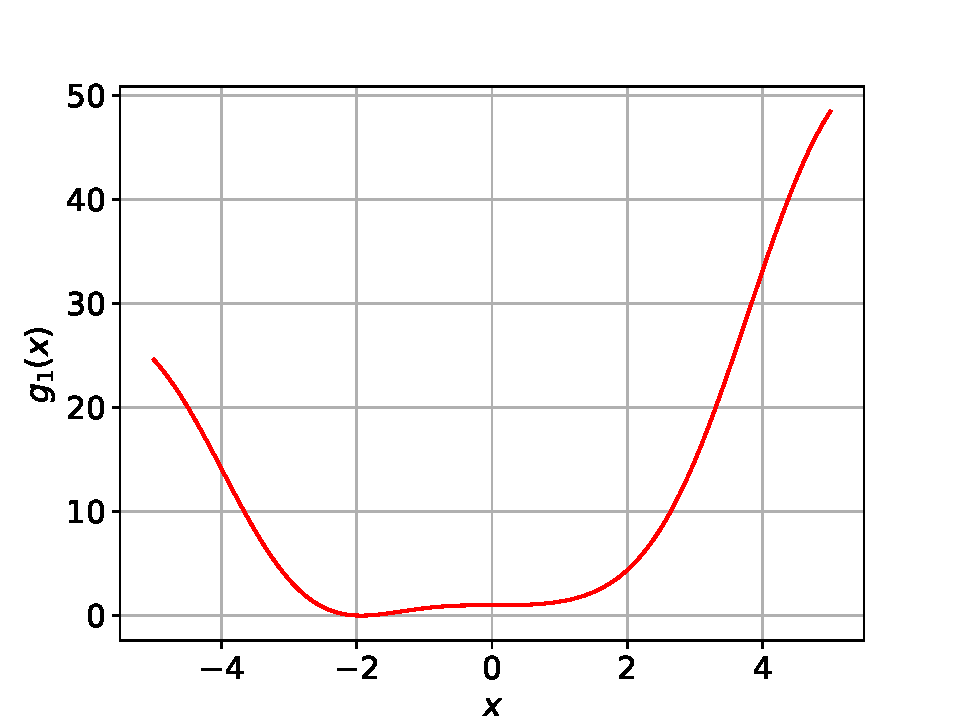
\includegraphics[width=0.6\textwidth]{Bisectoin_Question2.pdf}
  \caption{$g_1(x)$ Graph}
\end{figure}

\noindent  
BIsection Method의 코드중 
\begin{lstlisting}[language=Python]
    if f(a_n) * f(b_n) >= 0:
        print("Bisection method fails.")
        return None
\end{lstlisting}
에 의하여 Bisection Method fails 가 출력된다. 즉, $f(a_n) * f(b_n) \geq 0$ 이 성립되었다는 것인데, question 3에서 주어진 범위에서 함수의 값을 보면, $ f(a_n) * f(b_n) \geq 0$이 성립되었다는 것을 볼 수 있고, 따라서 우리는 Bisection Method를 이용할 수 없는 함수인 것을 볼 수 있다. $f_1(x)$ 을 그려보면 Figure 8 과 같다. 이 경우에 검은 색 점은, Newton's Method를 이용하여 해를 구한 것이다. 이는 -2에서 1까지의 범위사이의 $ f(a_n) * f(b_n) \geq 0$이 성립하지 않기 때문에 위에서 $f_1(x)$ 해를 구했듯, Bisection Method를 이용할 수 있는 것이다.

\clearpage


\noindent  
Question 2에서 주어진 테이블을 완성하면 Table 1과 같다. 

\begin{figure}[!ht]
\centering
  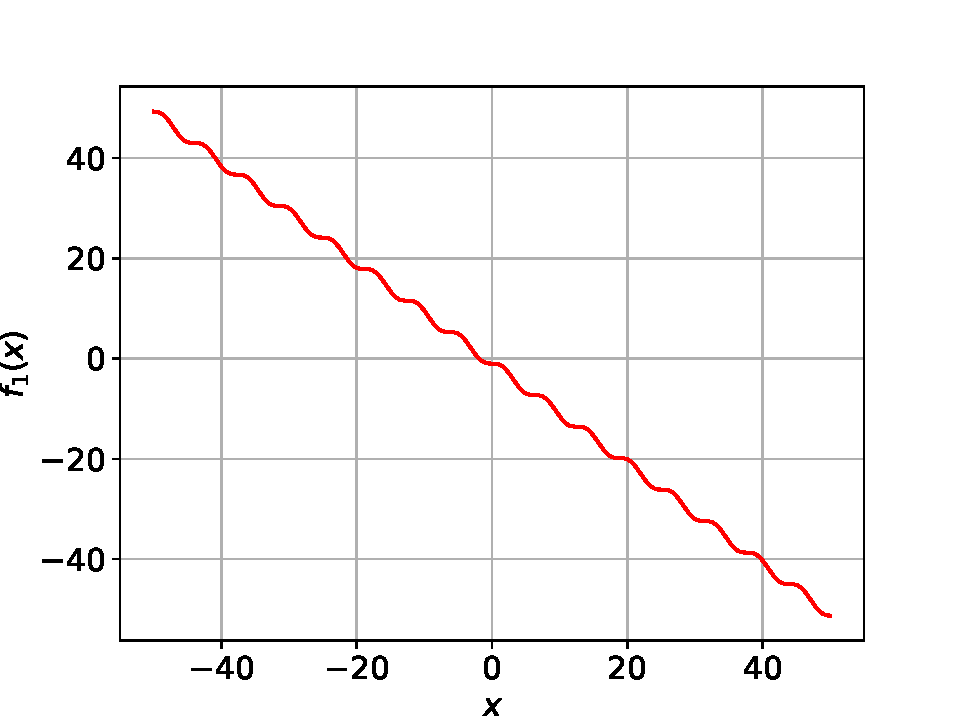
\includegraphics[width=0.6\textwidth]{Bisection_method1.pdf}
  \caption{$f_1(x)$ Graph}
\end{figure}

% Please add the following required packages to your document preamble:
% \usepackage{graphicx}
\begin{table}[]
\centering
\resizebox{\textwidth}{!}{%
\begin{tabular}{ccccc}
\hline
\multicolumn{1}{|c|}{}         & \multicolumn{2}{c|}{Bisection Method}                                        & \multicolumn{2}{c|}{Muller's Position}                                                              \\ \hline
\multicolumn{1}{|c|}{Function} & \multicolumn{1}{c|}{Num. Iters.} & \multicolumn{1}{c|}{Approx. Root}         & \multicolumn{1}{c|}{Num. Iters.} & \multicolumn{1}{c|}{Approx. Root}                                \\ \hline
\multicolumn{1}{|c|}{$f_1(x)$} & \multicolumn{1}{c|}{22}          & \multicolumn{1}{c|}{-1.934563398361206}   & \multicolumn{1}{c|}{5}           & \multicolumn{1}{c|}{0.816463380929969-1.563584661700659j}        \\ \hline
\multicolumn{1}{|c|}{$f_2(x)$} & \multicolumn{1}{c|}{22}          & \multicolumn{1}{c|}{2.384185791015625e-7} & \multicolumn{1}{c|}{14}          & \multicolumn{1}{c|}{-0.006364773235289123-0.007825774561814524j} \\ \hline
\multicolumn{1}{|c|}{$f_3(x)$} & \multicolumn{1}{c|}{22}          & \multicolumn{1}{c|}{0.25753092765808105}  & \multicolumn{1}{c|}{4}           & \multicolumn{1}{c|}{0.257530285446518+0j}                        \\ \hline
\multicolumn{1}{|c|}{}         & \multicolumn{2}{c|}{Newton's Method}                                         & \multicolumn{2}{c|}{Secant Method}                                                                  \\ \hline
\multicolumn{1}{|c|}{Function} & \multicolumn{1}{c|}{Num. Iters.} & \multicolumn{1}{c|}{Approx. Root}         & \multicolumn{1}{c|}{Num. Iters.} & \multicolumn{1}{c|}{Approx. Root}                                \\ \hline
\multicolumn{1}{|c|}{$f_1(x)$} & \multicolumn{1}{c|}{6}           & \multicolumn{1}{c|}{-1.9345632107520243}  & \multicolumn{1}{c|}{7}           & \multicolumn{1}{c|}{-1.9345632107520243}                         \\ \hline
\multicolumn{1}{|c|}{$f_2(x)$} & \multicolumn{1}{c|}{500}         & \multicolumn{1}{c|}{118.85559115473107}   & \multicolumn{1}{c|}{45}          & \multicolumn{1}{c|}{2.6043552455913054e-6}                       \\ \hline
\multicolumn{1}{|c|}{$f_3(x)$} & \multicolumn{1}{c|}{4}           & \multicolumn{1}{c|}{0.25753028543986073}  & \multicolumn{1}{c|}{5}           & \multicolumn{1}{c|}{0.2575302854398608}                          \\ \hline
\multicolumn{5}{c}{Table 1}                                                                                                                                                                                        
\end{tabular}%
}
\end{table}

















\section{Archimedes’ Law}
아르키메데스의 법칙을 식으로 표기하면 다음과 같다.
$$
\frac{1}{3}\pi (3rh^2 - h^3) \rho = \frac{4}{3}\pi r^3\sigma
$$

\noindent  
앞서 구한 방법대로 마찬가지로  optimize를 이용하여 Newton's Method로 코드를 구성하였다. 이때, $f(x)$ 에 관한 식으로 만들려면,  우변을 좌변으로 넘겨
$$
\frac{1}{3}\pi (3rh^2 - h^3) \rho - ( \frac{4}{3}\pi r^3\sigma ) = f(x) 
$$
로 만들어 준 뒤, 이를 def 함수로 나타내어 같은 방식으로 문제를 풀어주면 된다. 
\begin{lstlisting}[language=Python]
def arch(h) :
    r = 5
    p = 1
    o = 0.6
    return (1/3 * np.pi * (3 * r * h**2 - h**3) * p) - (4/3 * np.pi * r**3 * o)

def fprime(h):
    r = 5
    p = 1
    o = 0.6
    return 1/3 * np.pi * (6 * r * h - 3 * h**2) * p

sol = optimize.root_scalar(arch, x0 = 2, fprime = fprime, 
                          method='newton')
sol.root
Output : 5.670689228522684
\end{lstlisting}

이때 초기값에 따라 근이 세 개가 나올 수 있다. 당연히, h에 대한 삼차 방정식이기 때문에 해가 3개가 나오는 것은 당연하다. 또한 이는 위에서 언급한 Newton's Method의 단점 중 하나이다. 초기값을 어디로 설정하느냐에 따라서 수렴하는 해가 달라지게 된다. 즉, Figure 9 에서 볼 수 있는 $x$ 절편의 값 중 하나가 Solution이 된다.

\begin{figure}[!ht]
  \centering
  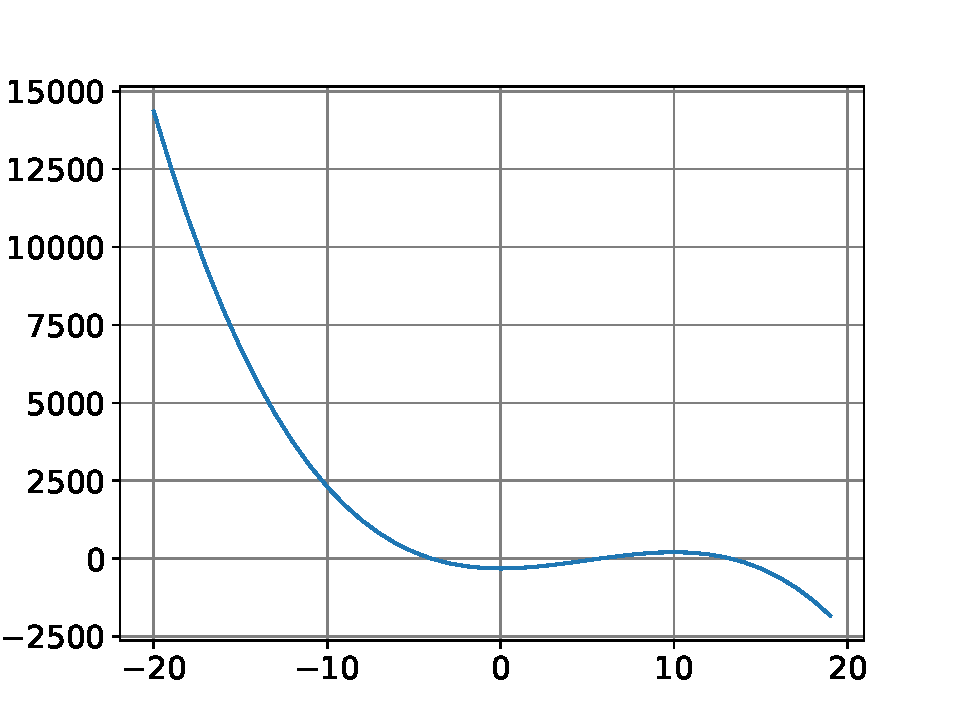
\includegraphics[width=0.55\textwidth]{Newton_Method3.pdf}
  \caption{$g_1(x)$ Graph}
\end{figure}

즉 초기값을 $x_0 = -3$ 으로 둘 경우 -3.976098746225619, $x_0 = 3$은 5.670689228522683, $x_0 = 11$ 은 13.305409517702934 이렇게 예상한대로 값을 추정할 수 있다. 그러나 h는 음수가 될 수 없으므로, 따라서 초기값을 $x_0 = 3$로 잡으면 5.670689228522683, $x_0 = 11$로 잡으면 13.305409517702934 이다.
\clearpage



\section{Discussion}
\subsection{함수에 대한 이해} 





















\end{document}
